\chapter{Diagramas internos de la \emph{FPGA}}
\label{ch:diagramas}

%* Diagrama TOP
\begin{figure}[p]
    \centering
    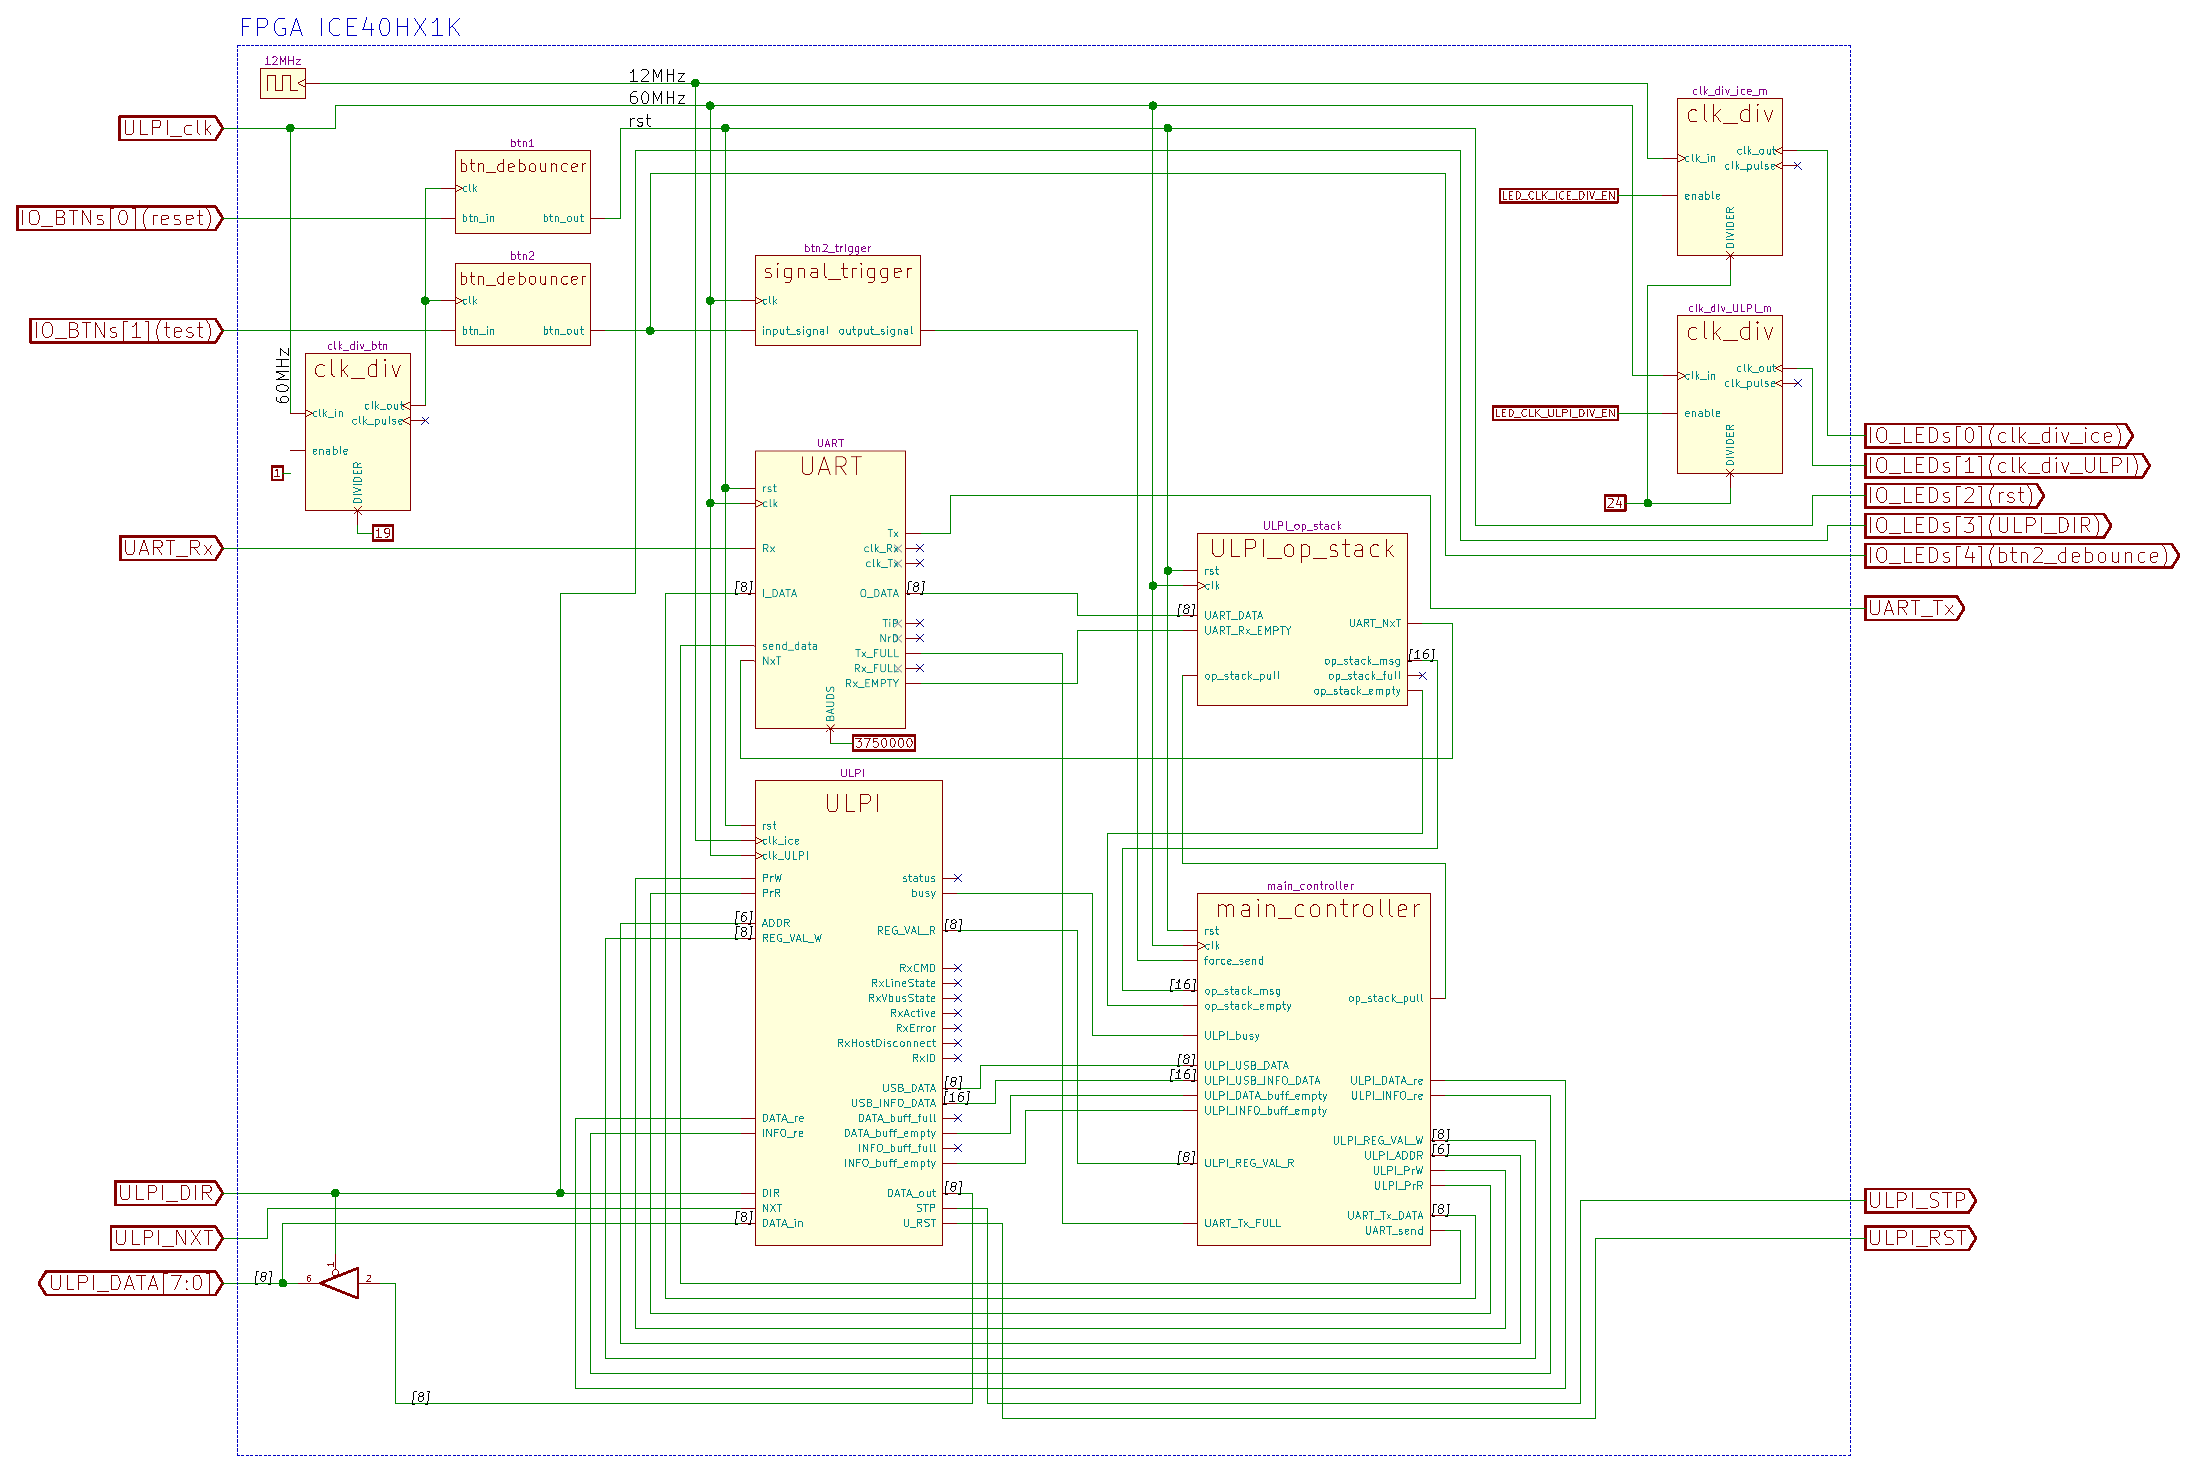
\includegraphics[rotate=90, width=150mm]{diagramas_FPGA/top.eps}
    \caption{Esquema principal usado en la \emph{FPGA}.}
    \label{fig:diagrama_fgpa_top}
\end{figure}

%* Diagrama UART_main
\begin{figure}[p]
    \centering
    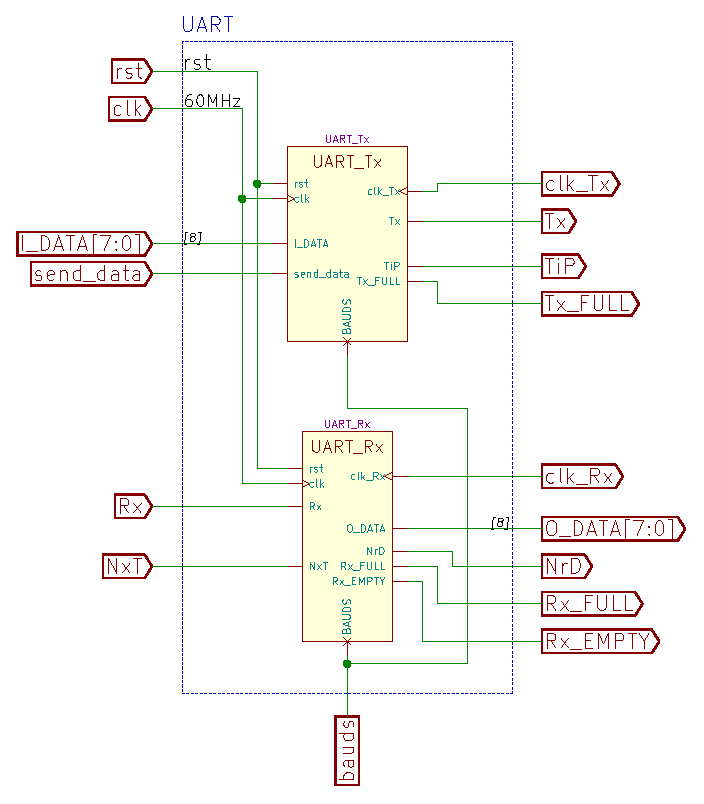
\includegraphics[rotate=90, width=150mm]{diagramas_FPGA/UART-UART.eps}
    \caption{Esquema principal del módulo de comunicación serie.}
    \label{fig:diagrama_fgpa_uart_main}
\end{figure}

%* Diagrama UART_Tx
\begin{figure}[p]
    \centering
    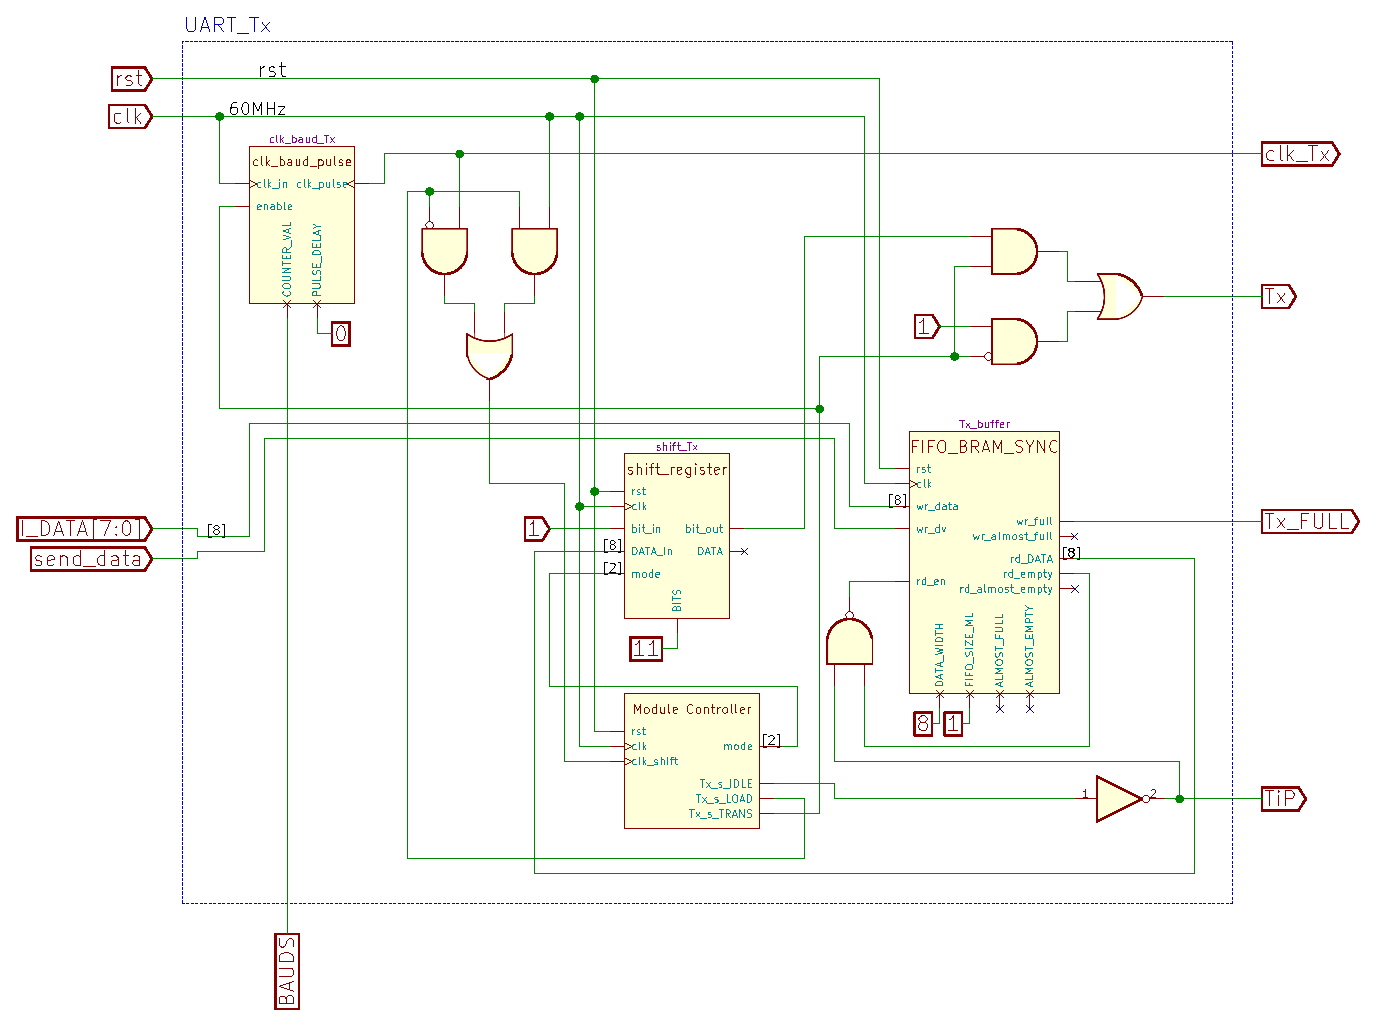
\includegraphics[rotate=90, width=150mm]{diagramas_FPGA/UART_Tx-UART-UART_Tx.eps}
    \caption{Esquema del submódulo de transmisión serie.}
    \label{fig:diagrama_fgpa_uart_tx}
\end{figure}

%* Diagrama UART_Rx
\begin{figure}[p]
    \centering
    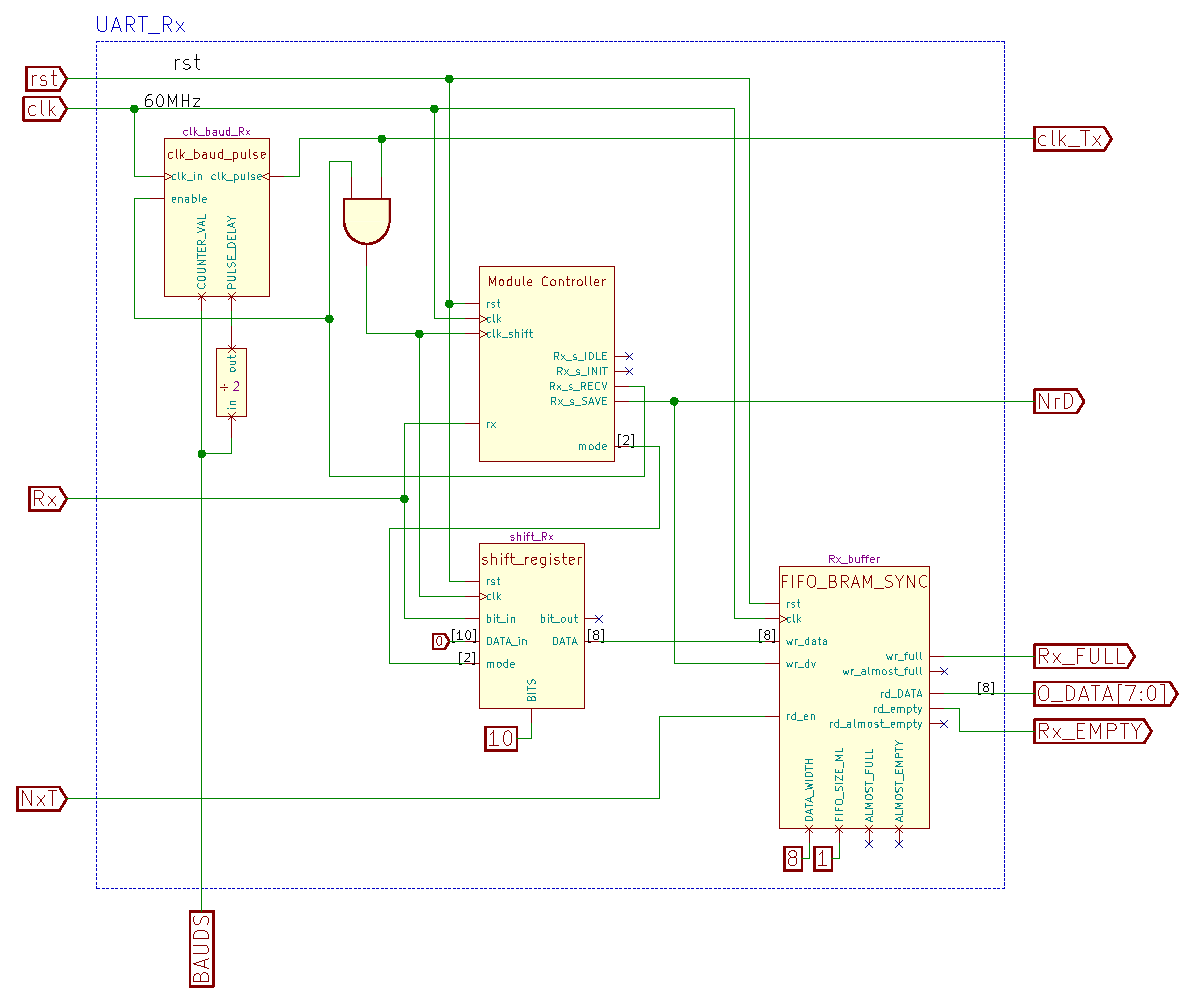
\includegraphics[rotate=90, width=150mm]{diagramas_FPGA/UART_Rx-UART-UART_Rx.eps}
    \caption{Esquema del submódulo de recepción serie.}
    \label{fig:diagrama_fgpa_uart_rx}
\end{figure}

%* Diagrama ULPI_main
\begin{figure}[p]
    \centering
    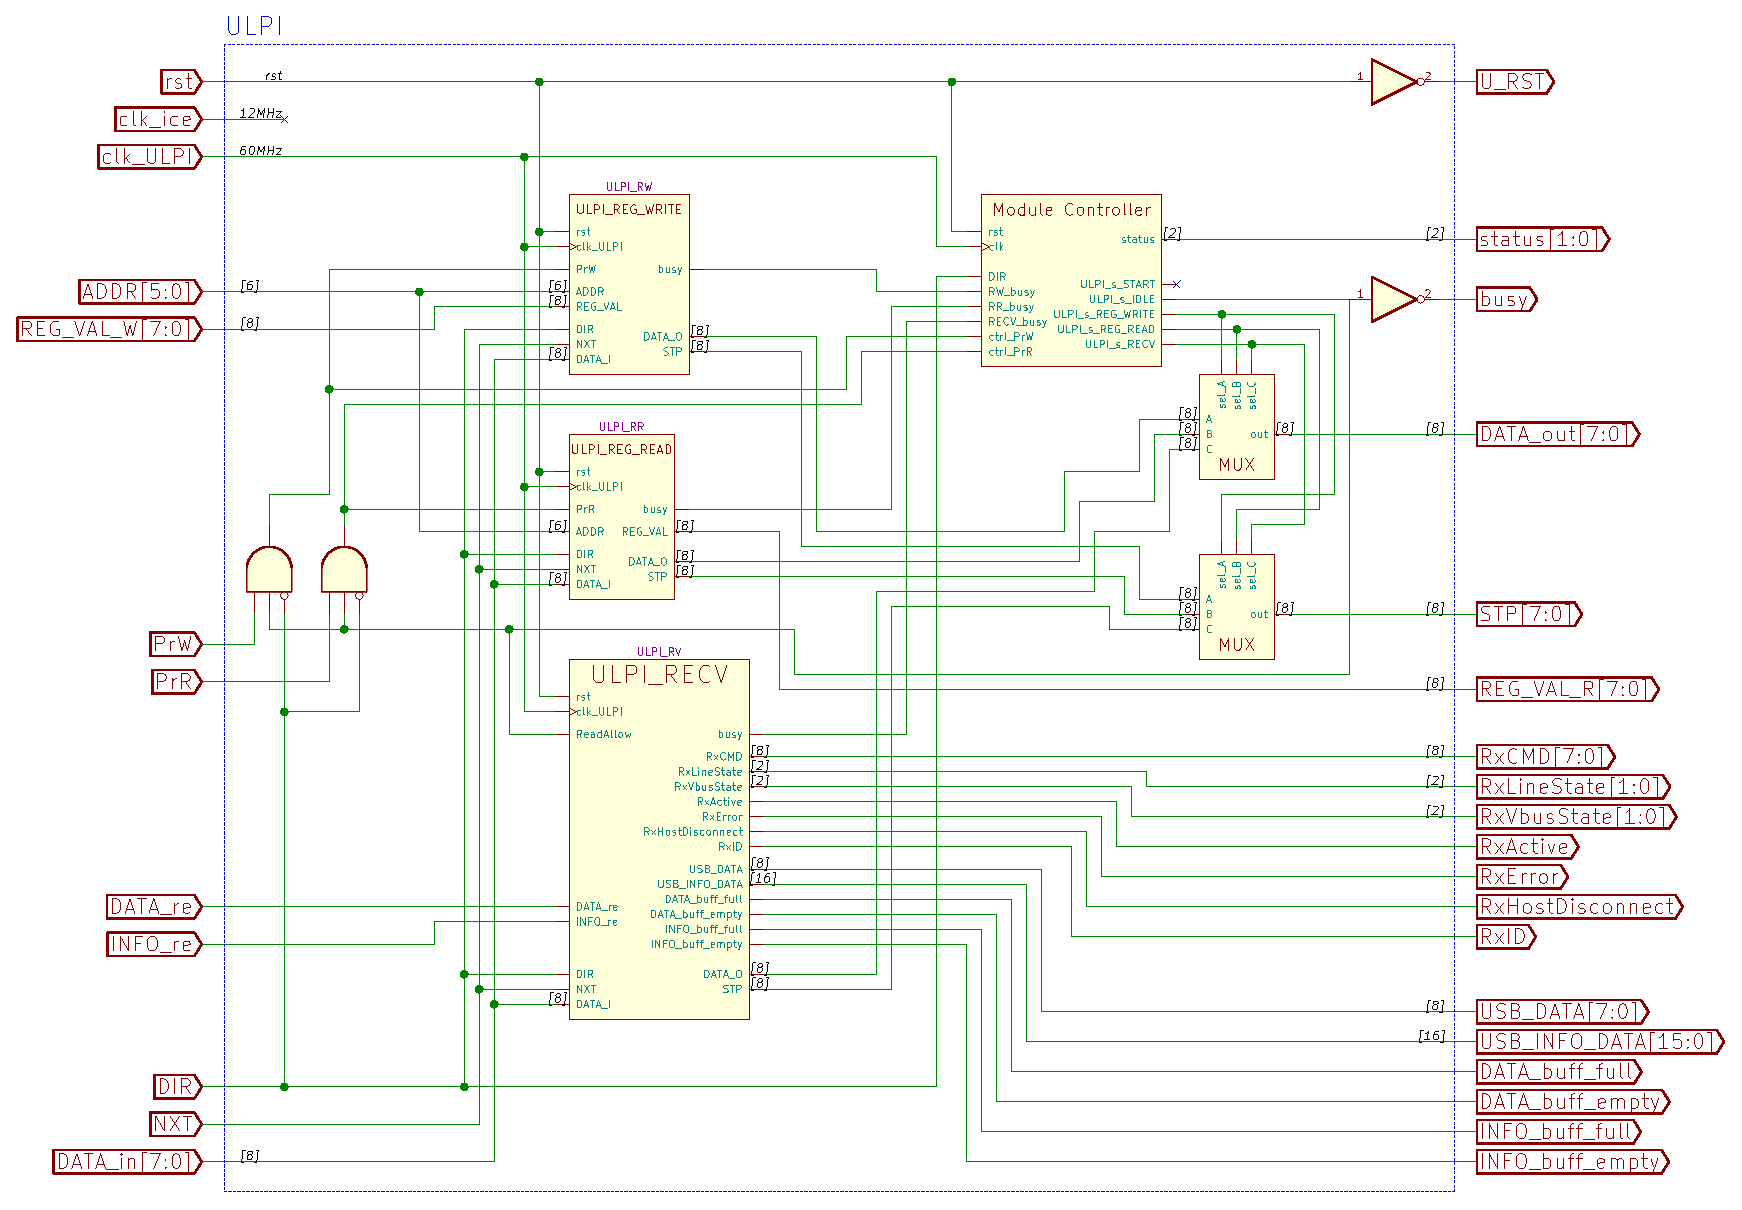
\includegraphics[rotate=90, width=150mm]{diagramas_FPGA/ULPI-ULPI.eps}
    \caption{Esquema principal del módulo de comunicación \emph{ULPI}.}
    \label{fig:diagrama_fgpa_ulpi_main}
\end{figure}

%* Diagrama ULPI_reg_rrite
\begin{figure}[p]
    \centering
    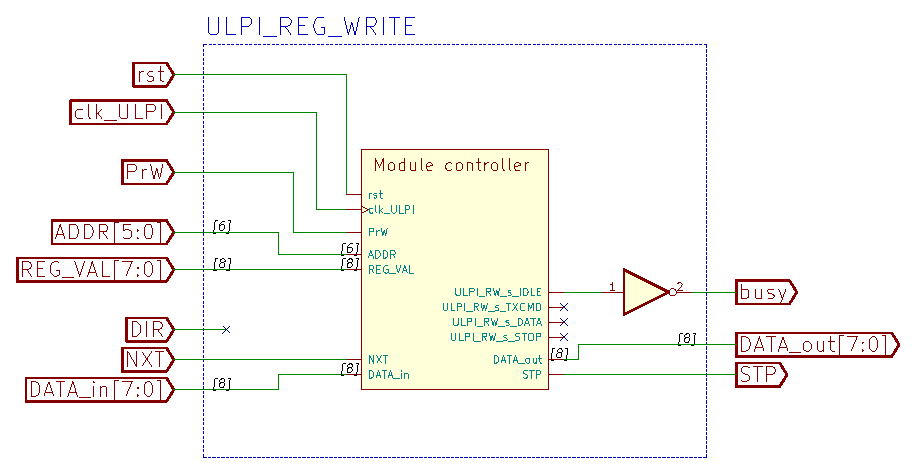
\includegraphics[rotate=90, width=95mm]{diagramas_FPGA/ULPI_REG_WRITE-ULPI-ULPI_REG_WRITE.eps}
    \caption{Esquema del submódulo de escritura de registros \emph{ULPI}.}
    \label{fig:diagrama_fgpa_ulpi_reg_write}
\end{figure}

%* Diagrama ULPI_reg_read
\begin{figure}[p]
    \centering
    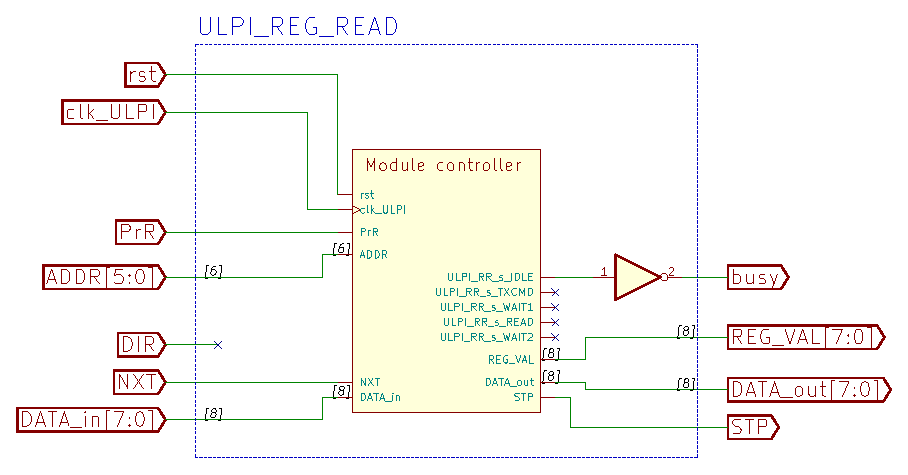
\includegraphics[rotate=90, width=95mm]{diagramas_FPGA/ULPI_REG_READ-ULPI-ULPI_REG_READ.eps}
    \caption{Esquema del submódulo de lectura de registros \emph{ULPI}.}
    \label{fig:diagrama_fgpa_ulpi_reg_read}
\end{figure}

%* Diagrama ULPI_recv
\begin{figure}[p]
    \centering
    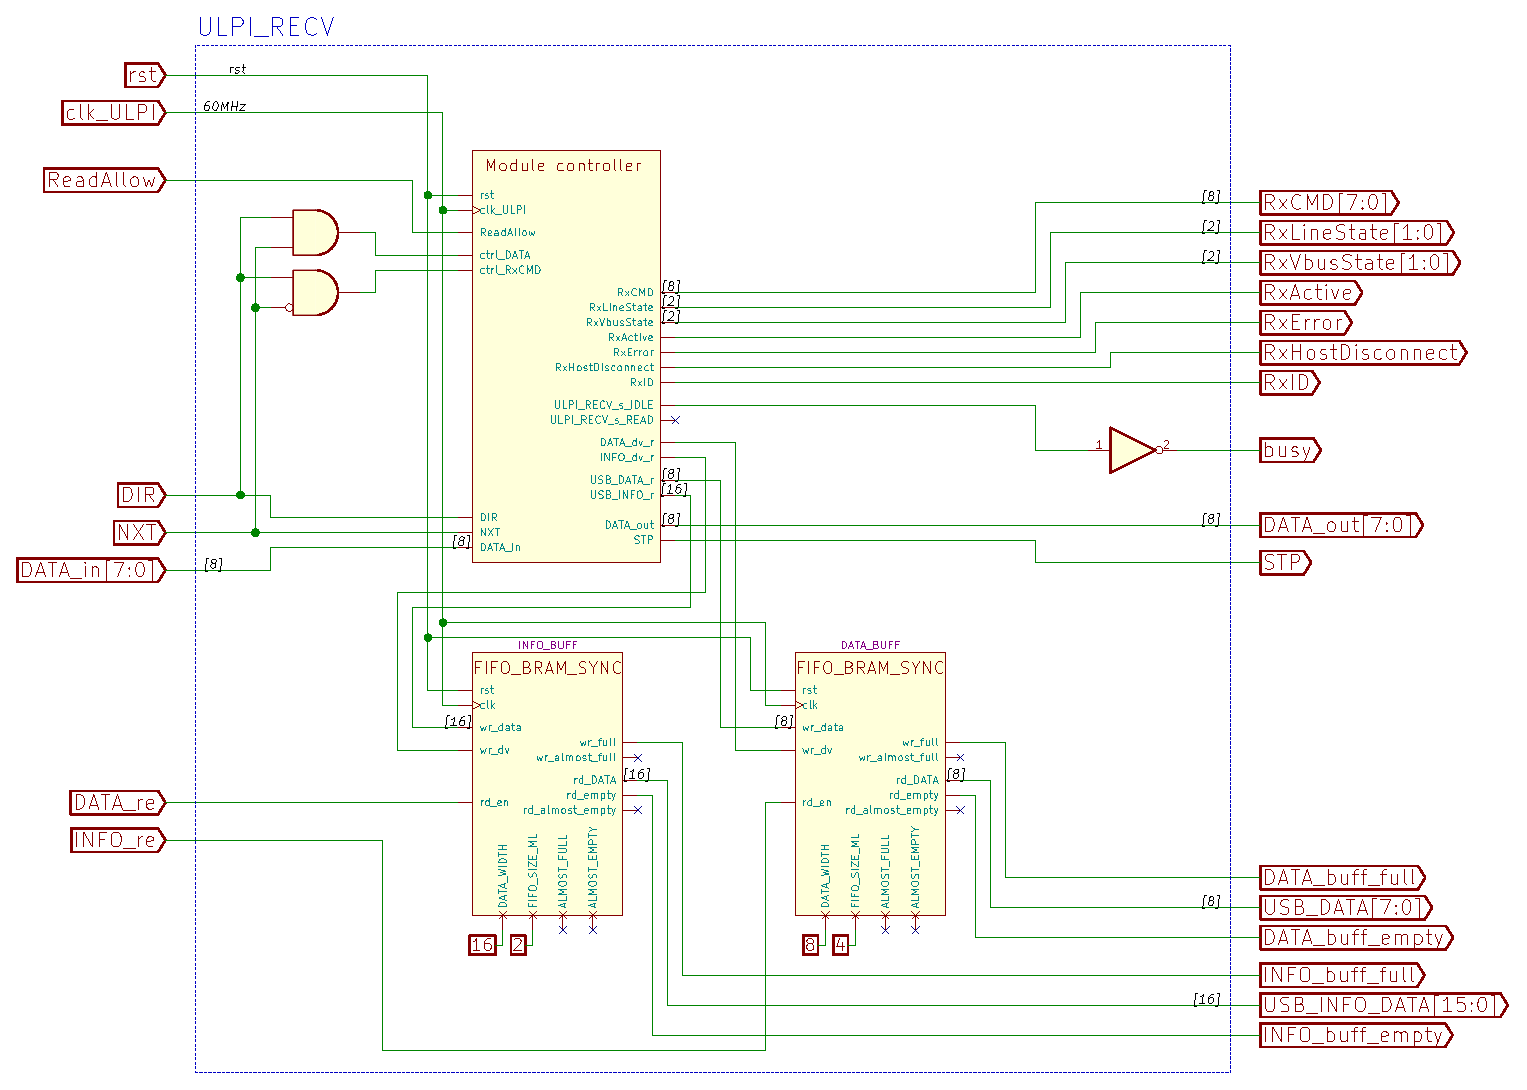
\includegraphics[rotate=90, width=150mm]{diagramas_FPGA/ULPI_RECV-ULPI-ULPI_RECV.eps}
    \caption{Esquema del submódulo de recpción de datos \emph{USB} a través de \emph{ULPI}.}
    \label{fig:diagrama_fgpa_ulpi_recv}
\end{figure}

%* Diagrama OP_buffer
\begin{figure}[p]
    \centering
    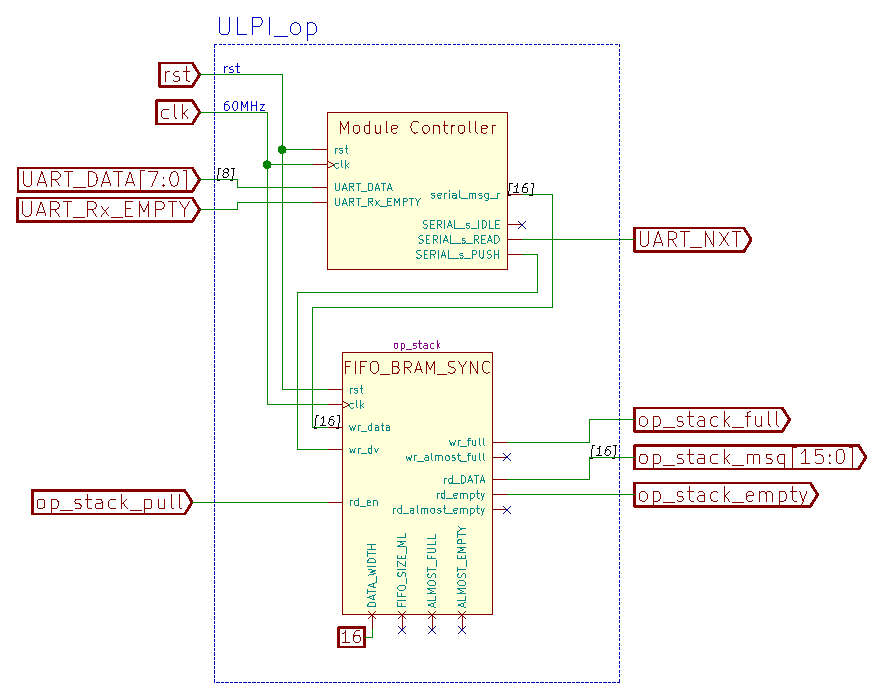
\includegraphics[rotate=90, width=150mm]{diagramas_FPGA/ULPI_op-ULPI_op.eps}
    \caption{Esquema del módulo de almacenaje de las operaciones pendientes.}
    \label{fig:diagrama_fgpa_op}
\end{figure}